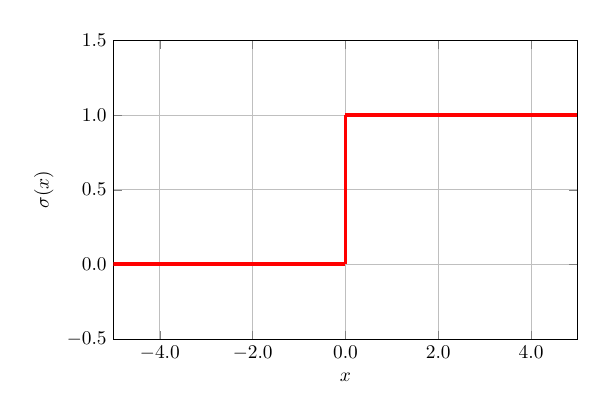
\begin{tikzpicture}[scale=0.70]
    \begin{axis}[
        width=10cm, height=7cm,
        xmin=-5, xmax=5,
        ymin=-0.5, ymax=1.5, 
        grid, 
        xlabel=$x$, ylabel=$\sigma(x)$,
        xtick = {-4.0,-2.0,0,2.0,4.0},
        ytick = {-0.5,0,0.5,1.0,1.5},
        y tick label style={/pgf/number format/.cd,%
                fixed,
                fixed zerofill,
                precision=1},
        x tick label style={/pgf/number format/.cd,%
                fixed,
                fixed zerofill,
                precision=1}
        ]
        
        \draw[line width=2.pt,color=red] (-5,0) -- (0,0);
        \draw[line width=2.pt,color=red] (0,0) -- (0,1);
        \draw[line width=2.pt,color=red] (0,1) -- (5,1);
        
    \end{axis}
\end{tikzpicture}